\documentclass[11pt]{article}
\usepackage[margin=0.78in]{geometry}
\usepackage[T1]{fontenc}
\usepackage[utf8]{inputenc}
\usepackage{lmodern}
\usepackage{microtype}
\usepackage{amsmath,amssymb,mathtools}
\usepackage{booktabs,array,longtable,multicol,enumitem}
\usepackage{xcolor}
\usepackage{hyperref}
\usepackage{tikz}
\usepackage[most]{tcolorbox}
\usetikzlibrary{arrows.meta,positioning,calc,shapes.geometric}
\hypersetup{colorlinks=true,linkcolor=blue!50!black,urlcolor=blue!50!black,pdftitle={Electrical Engineering Basics to Advanced: Inverter Systems Integration}}
\setlength{\parskip}{3pt}
\setlength{\parindent}{0pt}
\setlist[itemize]{topsep=2pt,itemsep=2pt,leftmargin=*}
\setlist[enumerate]{topsep=2pt,itemsep=3pt,leftmargin=*}
\renewcommand{\arraystretch}{1.16}
\setcounter{tocdepth}{2}
\definecolor{MSBlue}{RGB}{19,72,112}
\definecolor{MSGreen}{RGB}{25,112,85}
\definecolor{SoftBlue}{RGB}{237,246,253}
\definecolor{SoftGreen}{RGB}{238,249,242}
\definecolor{SoftYellow}{RGB}{255,249,231}
\definecolor{SoftRed}{RGB}{255,241,240}
\newtcolorbox{keybox}[1]{enhanced,breakable,colback=SoftBlue,colframe=MSBlue,title=\textbf{#1},arc=1.5mm,boxrule=0.65pt}
\newtcolorbox{examplebox}[1]{enhanced,breakable,colback=SoftYellow,colframe=orange!65!black,title=\textbf{Worked example: #1},arc=1.5mm,boxrule=0.65pt}
\newtcolorbox{warningbox}[1]{enhanced,breakable,colback=SoftRed,colframe=red!55!black,title=\textbf{Safety / integration caution: #1},arc=1.5mm,boxrule=0.65pt}
\newtcolorbox{checklistbox}[1]{enhanced,breakable,colback=SoftGreen,colframe=MSGreen,title=\textbf{#1},arc=1.5mm,boxrule=0.65pt}
\newcommand{\V}{\mathrm{V}}
\newcommand{\A}{\mathrm{A}}
\newcommand{\Hz}{\mathrm{Hz}}
\newcommand{\W}{\mathrm{W}}
\newcommand{\kW}{\mathrm{kW}}
\newcommand{\MW}{\mathrm{MW}}
\newcommand{\kVA}{\mathrm{kVA}}
\newcommand{\MVA}{\mathrm{MVA}}
\newcommand{\Mvar}{\mathrm{Mvar}}
\newcommand{\ohm}{\Omega}
\newcommand{\pu}{\mathrm{pu}}
\newcommand{\jop}{\mathrm{j}}
\title{\textbf{Electrical Engineering Basics to Advanced}\\\large Inverter Systems Integration Engineer Study Guide}
\author{Power Conversion, Grid Integration, Validation, and Field Diagnostics}
\date{\today}
\begin{document}
\maketitle
\begin{abstract}
This reference develops electrical engineering knowledge for integration of industrial, grid-interactive inverters with high-power generation assets and customer grids.
\end{abstract}
\tableofcontents
\newpage
\section{Role Context and System Boundary}

The core task is to deliver commanded real power safely and predictably while
respecting inverter, source, grid, protection, thermal, and regulatory limits.
The inverter is not an isolated box: control loops, cable impedance,
transformer vector groups, switchgear, utility source impedance, and plant
controls jointly determine its behavior.

\begin{figure}[h]
\centering
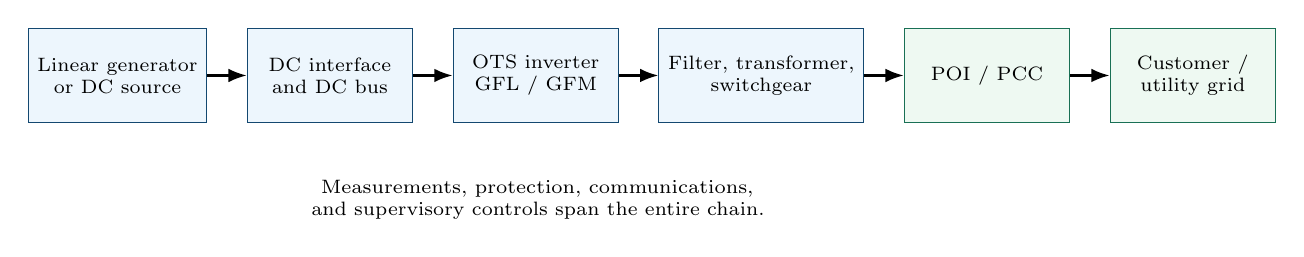
\begin{tikzpicture}[>=Latex,node distance=5mm,every node/.style={font=\scriptsize}]
\tikzset{block/.style={draw=MSBlue,fill=SoftBlue,minimum width=21mm,minimum height=12mm,align=center},grid/.style={draw=MSGreen,fill=SoftGreen,minimum width=21mm,minimum height=12mm,align=center}}
\node[block] (source) {Linear generator\\or DC source};
\node[block,right=of source] (dc) {DC interface\\and DC bus};
\node[block,right=of dc] (inv) {OTS inverter\\GFL / GFM};
\node[block,right=of inv] (ac) {Filter, transformer,\\switchgear};
\node[grid,right=of ac] (poi) {POI / PCC};
\node[grid,right=of poi] (utility) {Customer /\\utility grid};
\draw[->,thick] (source)--(dc);
\draw[->,thick] (dc)--(inv);
\draw[->,thick] (inv)--(ac);
\draw[->,thick] (ac)--(poi);
\draw[->,thick] (poi)--(utility);
\node[below=6mm of inv,align=center,text width=57mm] {Measurements, protection, communications, and supervisory controls span the entire chain.};
\end{tikzpicture}
\caption{Power-delivery system boundary. A decision in one block changes adjacent behavior.}
\end{figure}

\begin{longtable}{p{0.21\linewidth}p{0.36\linewidth}p{0.33\linewidth}}
\toprule
Lifecycle phase & Engineer deliverables & Completion evidence \\
\midrule
Requirements & Electrical envelope, grid-code matrix, interfaces & Approved limits, assumptions, pass/fail criteria \\
Selection and design & Sizing, protection, thermal, communications decisions & Design review with derating and fault calculations \\
Lab validation & Configuration baseline and test procedure & Repeatable data against requirements \\
Commissioning & Site settings and functional test records & Controlled configuration and signed evidence \\
Fleet support & Trend monitoring, RCA, corrective actions & Regression evidence and fleet screening \\
\bottomrule
\end{longtable}

\subsection{Essential terminology}
\begin{multicols}{2}
\begin{itemize}
\item \textbf{POI/PCC}: point of interconnection/common coupling.
\item \textbf{GFL}: grid-following; uses the grid as a voltage-angle reference.
\item \textbf{GFM}: grid-forming; establishes a controlled voltage-angle reference.
\item \textbf{LVRT}: low-voltage ride-through.
\item \textbf{SCR}: short-circuit ratio, a grid-strength screening measure.
\item \textbf{THD}: total harmonic distortion.
\item \textbf{OCPD}: overcurrent protective device.
\item \textbf{RMS}: heating-equivalent value of a waveform.
\end{itemize}
\end{multicols}

\section{Circuit, Energy, and Measurement Fundamentals}

\subsection{Voltage, current, power, and energy}
Voltage is potential difference and current is charge flow. With the passive
sign convention, instantaneous power is $p(t)=v(t)i(t)$. Positive average
power means a device absorbs energy. Energy transferred in time interval
$[t_1,t_2]$ is
\[
E=\int_{t_1}^{t_2}p(t)\,dt.
\]
For basic elements:
\[
v_R=Ri,\qquad i_C=C\frac{dv_C}{dt},\qquad v_L=L\frac{di_L}{dt}.
\]
The stored energies are $E_C=\frac12Cv_C^2$ and $E_L=\frac12Li_L^2$.
Capacitors oppose abrupt voltage changes; inductors oppose abrupt current
changes. These facts govern DC-bus excursions, inrush, and switching overshoot.

\begin{examplebox}{DC-bus power imbalance}
A $10\,\mathrm{mF}$ DC-link capacitor rises from $1000\,\V$ to $1050\,\V$:
\[
\Delta E=\frac12C(V_2^2-V_1^2)=0.5(0.010)(1050^2-1000^2)=512.5\,\mathrm{J}.
\]
At $100\,\kW$, this energy corresponds to only $5.1\,\mathrm{ms}$ of power
imbalance. High-power DC-bus controls and protection must respond rapidly.
\end{examplebox}

\subsection{Kirchhoff's laws and equivalent circuits}
Kirchhoff's current law says the algebraic current sum at a node is zero;
Kirchhoff's voltage law says the algebraic voltage sum around a closed loop is
zero. A useful grid model is a Thevenin voltage source behind impedance:
\[
\underline V_{POI}=\underline V_{th}-\underline I\underline Z_{th}.
\]
The grid is therefore not ideal. High source impedance makes POI voltage more
sensitive to inverter current and increases the chance of control interaction.

\subsection{RMS, crest factor, bandwidth, and safe probing}
For periodic $x(t)$ of period $T$,
\[
X_{rms}=\sqrt{\frac1T\int_0^T x^2(t)dt}.
\]
For a sine, $V_{rms}=\hat V/\sqrt2$. Crest factor is peak divided by RMS and
is larger for pulsed/fault currents than for a sine. Match probe, sensor, and
data-acquisition bandwidth to the phenomenon: a quality meter establishes
trends but cannot replace a high-bandwidth differential probe for switching
transients.

\begin{warningbox}{High-voltage instrumentation}
At 400--800 Vac and up to 1500 Vdc, use rated probes, leads, PPE, barriers,
and an approved energized-work process. Verify probe category, voltage rating,
common-mode limit, grounding scheme, and scope isolation before connection. A
bench-scope earth lead can create a dangerous unintended ground path.
\end{warningbox}

\subsection{Phasors and impedance}
At one sinusoidal frequency,
\[
v(t)=\sqrt2\Re\{\underline V e^{\jop\omega t}\},\qquad
\underline Z_R=R,\quad \underline Z_L=\jop\omega L,\quad
\underline Z_C=\frac{1}{\jop\omega C}.
\]
Phasors are excellent for fundamental power flow and faults, but do not by
themselves represent PWM switching, saturation, or discrete control states.

\section{AC, Three-Phase Power, and Per-Unit Analysis}

\subsection{Complex power}
For RMS phasors,
\[
\underline S=\underline V\underline I^*=P+\jop Q,\qquad |\underline S|^2=P^2+Q^2.
\]
$P$ is real power (W), $Q$ reactive power (var), and $|S|$ apparent power
(VA). $\mathrm{PF}=P/|S|=\cos\phi$. Most conventions use positive $Q$ for
inductive reactive absorption, but always verify the vendor's sign convention.

\subsection{Balanced three-phase systems}
\[
P=\sqrt3V_{LL}I_L\cos\phi,\qquad Q=\sqrt3V_{LL}I_L\sin\phi,\qquad
|S|=\sqrt3V_{LL}I_L.
\]
For wye, $V_{LL}=\sqrt3V_{LN}$ and $I_L=I_\phi$. For delta,
$V_{LL}=V_\phi$ and $I_L=\sqrt3I_\phi$. Three-wire systems can carry balanced
power without a neutral, but unbalance and ground faults depend on the actual
grounding and transformer connection.

\begin{examplebox}{Inverter AC current}
An inverter exports $1.00\,\MW$ at $480\,\V_{LL}$ and PF $=0.95$:
\[
S=\frac{P}{PF}=1.053\,\MVA,\qquad I=\frac{S}{\sqrt3V_{LL}}
=\frac{1.053\times10^6}{\sqrt3(480)}=1267\,\A.
\]
This is fundamental continuous current before overload, harmonics, ambient
derating, conductor/terminal limits, and equipment-listing conditions.
\end{examplebox}

\subsection{Power flow intuition and per-unit}
Across a mostly inductive connection with reactance $X$,
\[
P\approx\frac{V_1V_2}{X}\sin\delta.
\]
This motivates frequency--power droop. Reactive power is more linked to voltage
magnitudes. For per-unit analysis choose $S_B$ and $V_{B,LL}$:
\[
I_B=\frac{S_B}{\sqrt3V_{B,LL}},\qquad Z_B=\frac{V_{B,LL}^2}{S_B},\qquad
Z_{pu}=\frac{Z}{Z_B}.
\]
With voltage bases in the transformer ratio, transformer impedance has the same
numerical per-unit value on either side.

\begin{table}[h]
\centering
\caption{AC data and what a trend can indicate}
\begin{tabular}{p{0.25\linewidth}p{0.30\linewidth}p{0.34\linewidth}}
\toprule
Quantity & Typical source & Integration interpretation \\
\midrule
Voltage unbalance & Phase phasors or sequence components & Heating, PLL sensitivity, protection concerns \\
Frequency / ROCOF & PLL or independent estimator & Grid event, islanding, controller interaction \\
PF and kvar & Fundamental $P,Q,S$ & Reactive capability and volt-var operation \\
THD and harmonics & FFT with stated window/bandwidth & Filter resonance, nonlinear-load interaction \\
DC bus & Fast differential measurement / internal log & Source/load power mismatch and fault response \\
\bottomrule
\end{tabular}
\end{table}

\section{Transformers, Cables, Switchgear, and Grounding}

\subsection{Transformer behavior}
The ideal transformer obeys $V_1/V_2=N_1/N_2$ and $I_1/I_2=N_2/N_1$.
Real transformers add resistance, leakage reactance, magnetizing current,
core loss, taps, and thermal limits. Impedance limits fault current but also
causes voltage drop and phase lag. Vector group matters: delta--wye connections
can block zero-sequence transfer and introduce 30-degree displacement. Confirm
that relay, meter, inverter, and controller reference frames match reality.

An approximate voltage-regulation expression is
\[
\%VR\approx\frac{I(R\cos\phi+X\sin\phi)}{V}\times100\%.
\]

\subsection{Cables, bus, and current capacity}
Cable ampacity depends on conductor material, insulation and terminal ratings,
ambient temperature, installation method, grouping, and code-required derating.
At high current also consider AC resistance, skin/proximity effect, parallel
conductor sharing, bus-joint torque, and hot spots. Balanced three-phase voltage
drop is approximately
\[
\Delta V\approx\sqrt3I(R\cos\phi+X\sin\phi).
\]
Cable inductance that seems small at 60 Hz may strongly influence fast
current-control dynamics.

\subsection{Grounding, bonding, and switchgear}
Grounding establishes an earth/neutral reference; bonding creates a reliable
fault-current path between exposed conductive parts. Grounding method determines
line-to-ground fault current and relay strategy. Do not assume a neutral exists
or that a ground conductor carries normal load current. Switchgear selection
must include voltage, continuous current, available fault duty, interrupting
duty, making/latching duty, insulation, and installed application.

\begin{warningbox}{Standards and code}
NEC (NFPA 70), IEEE 1547, UL 1741, utility tariffs, and local amendments are
edition and jurisdiction specific. Use current adopted editions, manufacturer
listing instructions, and AHJ interpretation for conductor sizing, OCPD,
grounding/bonding, disconnects, labels, and commissioning. This guide provides
engineering concepts, not a compliance determination.
\end{warningbox}

\section{Power Electronics Hardware and the Inverter Plant}

\subsection{Voltage-source inverter architecture}
An integration engineer may not design semiconductor gates or PCB layouts, but
must understand the constraints they impose. A typical voltage-source inverter
(VSI) includes a DC link, semiconductor bridge, AC filter, measurement chain,
gate-drive and protection functions, cooling, and supervisory controls.

\begin{figure}[h]
\centering
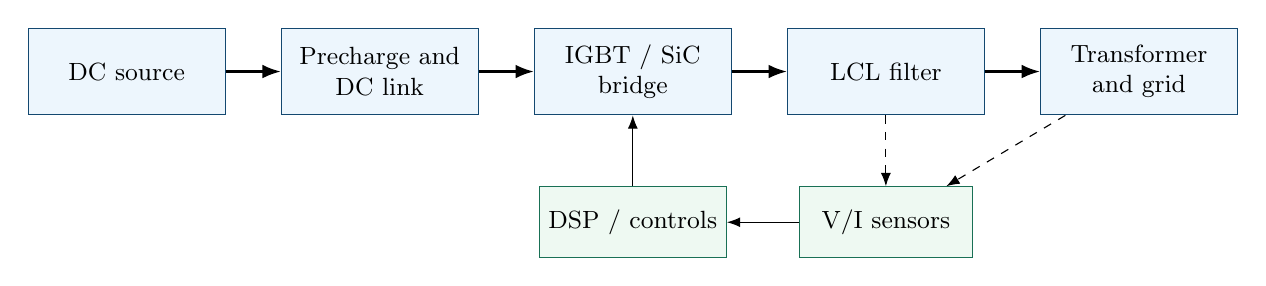
\begin{tikzpicture}[>=Latex,node distance=7mm,every node/.style={font=\small}]
\tikzset{pblock/.style={draw=MSBlue,fill=SoftBlue,minimum width=25mm,minimum height=11mm,align=center},sblock/.style={draw=MSGreen,fill=SoftGreen,minimum width=22mm,minimum height=9mm,align=center}}
\node[pblock] (src) {DC source};
\node[pblock,right=of src] (bus) {Precharge and\\DC link};
\node[pblock,right=of bus] (bridge) {IGBT / SiC\\bridge};
\node[pblock,right=of bridge] (filter) {LCL filter};
\node[pblock,right=of filter] (grid) {Transformer\\and grid};
\node[sblock,below=9mm of bridge] (ctrl) {DSP / controls};
\node[sblock,below=9mm of filter] (sense) {V/I sensors};
\draw[->,thick] (src)--(bus);
\draw[->,thick] (bus)--(bridge);
\draw[->,thick] (bridge)--(filter);
\draw[->,thick] (filter)--(grid);
\draw[->] (sense)--(ctrl);
\draw[->] (ctrl)--(bridge);
\draw[->,dashed] (filter)--(sense);
\draw[->,dashed] (grid)--(sense);
\end{tikzpicture}
\caption{Simplified voltage-source inverter and feedback paths.}
\end{figure}

\subsection{DC link and precharge}
The DC link buffers switching ripple and momentary source/load mismatch.
Precharge limits capacitor charging current before main-contactor closure.
Failed precharge, incorrect timing, or leaky capacitors can cause contactor
welding or startup faults. During an AC fault, reduced real-power export can
raise $V_{dc}$ unless the source is curtailed, energy is absorbed, or a defined
protective sequence acts.

\subsection{PWM, devices, and EMI}
Pulse-width modulation (PWM) synthesizes the AC fundamental from DC voltage.
Higher switching frequency can reduce current ripple and filter size but
normally increases switching loss and electromagnetic interference (EMI):
\[
P_{loss}\approx P_{cond}+P_{sw},\qquad P_{sw}\propto f_{sw}.
\]
Semiconductor capability depends on junction temperature, modulation index,
switching frequency, cooling, overload duration, safe-operating area, and
manufacturer protection behavior. A catalog current rating is not a complete
operating envelope.

\subsection{L, LC, and LCL filters}
An LCL filter attenuates PWM ripple more efficiently than a single inductor but
creates a resonance. An undamped resonance estimate is
\[
f_r=\frac{1}{2\pi}\sqrt{\frac{L_1+L_2}{L_1L_2C_f}}.
\]
Place resonance appropriately relative to the fundamental, switching frequency,
sampling/control delay, and expected grid inductance. Damping can be passive
(with loss) or active (model and measurement sensitive). Never tune an
LCL-controlled inverter only against one ideal grid condition.

\subsection{Thermal chain and derating}
The thermal chain is analogous to an RC network:
\[
T_j=T_a+P_{loss}(R_{\theta jc}+R_{\theta cs}+R_{\theta sa}).
\]
Real equipment includes time constants, fan curves, coolant temperature,
altitude effects, dust, and uneven heat sharing. Verify whether a vendor kVA
rating is continuous at the installed ambient, altitude, switching mode, grid
voltage, PF, and enclosure configuration.

\section{Grid-Following Control}

\subsection{Reference frames and phase-locked loop}
A GFL inverter measures grid voltage and estimates phase angle $\theta$ and
frequency $\omega$ using a PLL. A Park transform maps three-phase quantities
into a rotating $dq$ frame. When the $d$ axis aligns with grid voltage,
$v_q\approx0$; in one common convention, $i_d$ controls real power and $i_q$
controls reactive power. Axis and sign definitions vary by vendor, so verify
the actual parameter guide and telemetry mapping.

\begin{figure}[h]
\centering
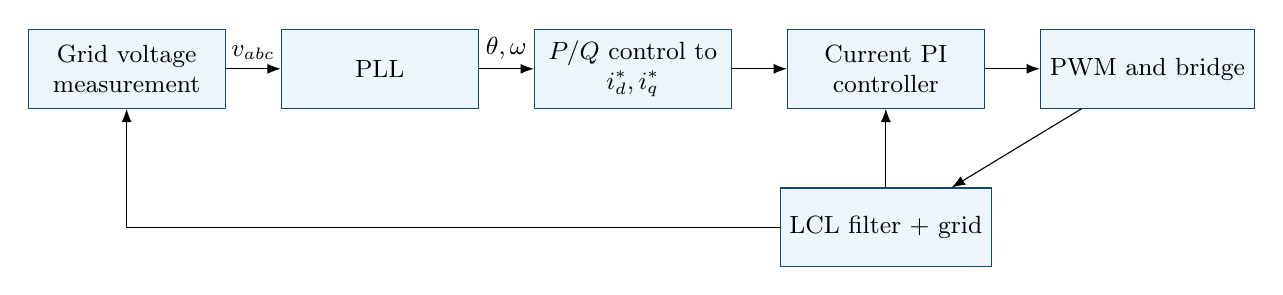
\begin{tikzpicture}[>=Latex,node distance=7mm,every node/.style={font=\small}]
\tikzset{cblock/.style={draw=MSBlue,fill=SoftBlue,minimum width=25mm,minimum height=10mm,align=center}}
\node[cblock] (measure) {Grid voltage\\measurement};
\node[cblock,right=of measure] (pll) {PLL};
\node[cblock,right=of pll] (outer) {$P/Q$ control to\\$i_d^*,i_q^*$};
\node[cblock,right=of outer] (inner) {Current PI\\controller};
\node[cblock,right=of inner] (pwm) {PWM and bridge};
\node[cblock,below=10mm of inner] (plant) {LCL filter + grid};
\draw[->] (measure)--node[above] {$v_{abc}$}(pll);
\draw[->] (pll)--node[above] {$\theta,\omega$}(outer);
\draw[->] (outer)--(inner);
\draw[->] (inner)--(pwm);
\draw[->] (pwm)--(plant);
\draw[->] (plant.west)-|(measure.south);
\draw[->] (plant.north)--(inner.south);
\end{tikzpicture}
\caption{Conceptual GFL hierarchy. Current control is faster than outer power control.}
\end{figure}

\subsection{Loop bandwidth and grid strength}
Control loops require separation in bandwidth: current loops are normally
fastest, DC-voltage/power loops slower, and plant supervisory logic slower
again. A PLL that is too fast can chase distorted voltage or interact with a
weak grid; too slow can impair transient tracking. Lowering PLL bandwidth is a
common weak-grid mitigation, but must be tested with actual filters, source
impedance, current limits, and ride-through logic.

Grid strength is often screened using
\[
\mathrm{SCR}=\frac{S_{sc}}{S_{inv,rated}},\qquad S_{sc}\approx\frac{V_{LL}^2}{|Z_{th}|}.
\]
SCR is useful but incomplete. $R/X$, resonances, multiple converters, cable
length, transformer saturation, and control settings can make two equal-SCR
systems behave differently.

\subsection{Current limits and anti-windup}
The converter command must remain inside its current capability circle:
\[
i_d^{*2}+i_q^{*2}\le i_{max}^2.
\]
During a voltage sag, reactive-current priority can leave less current for real
power. Firmware must define priority, clipping, and anti-windup behavior.
Integrators must test the transition itself: a controller integrator that winds
up while the output is limited can cause overshoot or nuisance trips when the
event clears.

\section{Grid-Forming Control and Islanded Operation}

\subsection{The grid-forming objective}
A GFM inverter behaves as a controllable voltage source behind impedance. It
sets voltage and frequency references instead of using a PLL as its primary
reference. This can strengthen a weak grid or support an island, but no inverter
can exceed DC-source energy, current, thermal, or protection constraints.

\subsection{Droop and virtual impedance}
One common steady-state droop formulation is
\[
\omega=\omega_0-m_p(P-P_0),\qquad V=V_0-n_q(Q-Q_0),
\]
where $m_p$ and $n_q$ are droop slopes. Compatible settings allow sources to
share load without high-speed communication. Droop that is too steep permits
large voltage/frequency movement; too shallow can cause poor sharing or control
conflict.

Virtual impedance adjusts voltage command in proportion to current:
\[
\underline V^*=\underline V_{ref}-\underline Z_v\underline I.
\]
It can improve sharing and damping but adds voltage drop and can impair
regulation. Converter fault current is normally controlled and limited near
rated current for a vendor-specific duration; it is not equivalent to large
synchronous-generator fault current.

\subsection{Transition and protection implications}
Coordinate grid-to-island and resynchronization transitions with breaker state,
phase/frequency/voltage matching, load step, current limits, protection groups,
and DC-source constraints. A no-load transition does not establish that the
system handles nonlinear load, motor start, or a large step load.

\begin{checklistbox}{GFM tuning questions}
\begin{itemize}
\item What establishes the reference and phase continuity during grid loss?
\item Which droop and virtual-impedance values apply in each operating mode?
\item How do current/DC limits and anti-windup change fault behavior?
\item How will parallel GFM sources avoid circulating reactive current?
\item Which protection functions remain dependable under limited fault current?
\end{itemize}
\end{checklistbox}

\section{Stability and Impedance-Based Thinking}

An inverter is a controlled, frequency-dependent source or load. The grid,
transformer, cable, filter, and adjacent converters present frequency-dependent
impedance. Oscillation can occur if loop gain is high where phase lag approaches
$-180^\circ$, or when source/load impedances interact adversely. Symptoms
include sustained ringing, harmonic sidebands, repetitive trips, or sensitivity
to cable length and grid strength.

For open-loop transfer function $L(s)$, closed-loop response is
\[
T(s)=\frac{L(s)}{1+L(s)}.
\]
Gain and phase margins are useful robustness indicators, but interpret them with
delay, nonlinear limits, parameter variation, and the complete operating range.

\begin{enumerate}
\item Establish topology, transformer vector group, cable/filter values, and source Thevenin range.
\item Identify vendor-approved PLL, current-loop, droop, damping, and limiter settings.
\item Screen worst credible grid strength, $R/X$, operating point, and parallel-source state.
\item Use simulation, impedance scans, or controlled steps to locate weakly damped modes.
\item Change one parameter family at a time; record configuration and waveforms.
\item Revalidate normal operation, disturbances, protective limits, and recovery.
\end{enumerate}

\section{Interconnection Functions and Grid-Code Validation}

\subsection{Translate requirements into evidence}
IEEE 1547 describes distributed-energy-resource interconnection and
interoperability requirements; UL 1741 is an equipment certification and
evaluation framework; utilities add location-specific settings and studies.
Translate every applicable requirement into a test matrix: condition,
measurement point, threshold, timer, required response, configuration source,
and evidence artifact. A generic factory default is not automatically acceptable
at a particular POI.

\begin{table}[h]
\centering
\caption{Representative interconnection behavior categories}
\begin{tabular}{p{0.23\linewidth}p{0.29\linewidth}p{0.36\linewidth}}
\toprule
Category & What is assessed & Integration evidence \\
\midrule
Voltage ride-through & Connection/trip regions, current response, recovery & Programmed curve, voltage/current trace, timers \\
Frequency response & Frequency-watt, thresholds, rate limits & Frequency profile and power response \\
Voltage regulation & Volt-var / volt-watt functions and priority & $V,Q,P$ curves and interaction check \\
Anti-islanding & Required response and site-mode coordination & Test method and relay/controller response \\
Power quality & Harmonics, flicker, DC injection, unbalance & Meter method, operating point, result \\
Communications & Read/write, reporting, control authority & Point map, permissions, timestamps \\
\bottomrule
\end{tabular}
\end{table}

\subsection{Voltage and frequency ride-through}
Ride-through is not merely ``do not trip.'' It specifies behavior through a
voltage/frequency profile, including timers, current injection or priority,
cease-to-energize regions, recovery ramps, and measurement filtering. Test
threshold tolerances, timer boundaries, repeated disturbances, phase-specific
events, recovery, and simultaneous frequency/voltage conditions.

\begin{figure}[h]
\centering
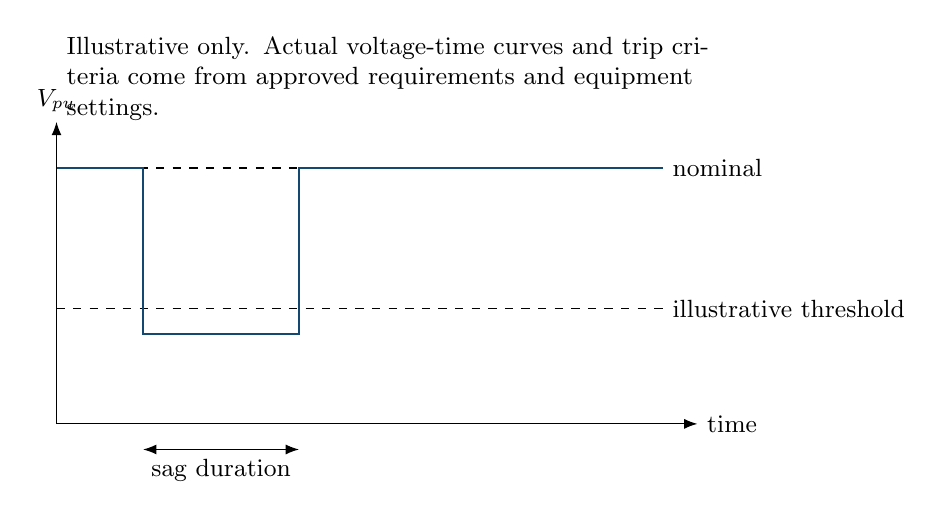
\begin{tikzpicture}[x=1.10cm,y=3.25cm,>=Latex,font=\small]
\draw[->] (0,0)--(7.4,0) node[right] {time};
\draw[->] (0,0)--(0,1.18) node[above] {$V_{pu}$};
\draw[dashed] (0,1)--(7,1) node[right] {nominal};
\draw[dashed] (0,.45)--(7,.45) node[right] {illustrative threshold};
\draw[thick,MSBlue] (0,1)--(1,1)--(1,.35)--(2.8,.35)--(2.8,1)--(7,1);
\draw[<->] (1,-.10)--(2.8,-.10) node[midway,below] {sag duration};
\node[align=left,text width=8.1cm] at (3.8,1.35) {Illustrative only. Actual voltage-time curves and trip criteria come from approved requirements and equipment settings.};
\iffalse
\node[align=left,text width=8.1cm] at (3.8,1.35) {Illustrative only. Actual voltage-time curves, current commands,\nand trip criteria come from approved requirements and equipment settings.};
\fi
\end{tikzpicture}
\caption{A voltage-sag profile used to organize an LVRT test.}
\end{figure}

\subsection{Voltage and reactive-power functions}
Volt-var control changes reactive power in response to voltage; volt-watt
reduces active power as voltage rises; frequency-watt changes active power in
response to frequency. Integration questions include deadbands, slopes, update
rate, ramp limits, reactive versus active priority, current saturation, and
interaction with feeder regulators/capacitor banks. Do not study an inverter
function in isolation when a utility regulator or plant controller also acts on
the same variable.

\section{Protection, Faults, and Symmetrical Components}

\subsection{Symmetrical components}
Unbalanced faults are analyzed with positive, negative, and zero sequence. Let
$a=e^{\jop120^\circ}$. Then
\[
\begin{bmatrix}V_a\\V_b\\V_c\end{bmatrix}=
\begin{bmatrix}1&1&1\\1&a^2&a\\1&a&a^2\end{bmatrix}
\begin{bmatrix}V_0\\V_1\\V_2\end{bmatrix}.
\]
Positive sequence is balanced normal rotation, negative sequence is balanced
reverse rotation, and zero sequence is in phase. Transformer connections and
grounding determine zero-sequence paths. Negative sequence can heat rotating
machines and affect controller/measurement behavior.

\subsection{Fault levels and inverter-limited current}
For a three-phase bolted fault, a first approximation is
\[
I_{3\phi}=\frac{V_{LL}}{\sqrt3|Z_{th}|}.
\]
Actual available fault current requires a complete network and time-dependent
source models. Inverters normally limit their fault current to a controlled
multiple near rated current for a short vendor-specific duration; they do not
behave like large synchronous machines. Protection coordination cannot assume
unlimited short-circuit contribution.

\begin{table}[h]
\centering
\caption{Common protective functions; ANSI device numbers are conventional labels}
\begin{tabular}{p{0.16\linewidth}p{0.25\linewidth}p{0.47\linewidth}}
\toprule
Function & Typical purpose & Integration concern \\
\midrule
27 / 59 & Under/overvoltage & Separate grid event, tap action, and local transient \\
81U / 81O & Under/overfrequency & Coordinate with frequency-watt and island mode \\
50 / 51 & Instantaneous/time overcurrent & May lack sensitivity with converter-limited fault current \\
67 & Directional overcurrent & Directional reference, polarity, transformer shift matter \\
32 & Directional power & Prevent undesired reverse power where required \\
25 & Synchronism check & Verify voltage, phase, and slip before close \\
87 & Differential & CT placement, ratio, saturation, restraint determine security \\
\bottomrule
\end{tabular}
\end{table}

\subsection{Protection coordination workflow}
Start with source and transformer data, grounding method, conductor/bus limits,
available fault duty, breaker/fuse curves, relay settings, and inverter fault
response. Study normal and minimum-source cases, not just maximum fault level.
Confirm selectivity, equipment protection, personnel safety, relay polarity,
and all control/protection state changes across GFL, GFM, and island modes.

\section{Power Quality and Waveform Analysis}

\subsection{Harmonics and distortion}
For voltage or current harmonics,
\[
\mathrm{THD}=\frac{\sqrt{\sum_{h=2}^{\infty}X_h^2}}{X_1}\times100\%.
\]
Always report the method: fundamental definition, aggregation interval,
bandwidth, operating point, instrument class, and measurement location.
Harmonic problems can come from PWM, LCL resonance, capacitor banks,
transformer saturation, nonlinear loads, or multiple-converter interaction.
Low total THD does not prove an important individual harmonic is absent.

\subsection{Flicker, unbalance, and transients}
Voltage flicker relates to perceptible modulation and requires standardized
measurement methods. Unbalance can be expressed with sequence components, for
example $|V_2|/|V_1|$. Transients include switching surges, lightning,
fault-clearing recovery, and breaker/contactor events. Triggered waveform
capture should include voltage, current, DC bus, gate/enable or state signals,
and a time-synchronized event log wherever possible.

\subsection{Waveform-first diagnosis}
Start with timing relationships, not one RMS number. Ask: Which phase leads?
Does current command change before current? Does the DC bus rise before the
trip? Is frequency estimate physical or PLL noise? Is ringing near an LCL,
cable, or capacitor-bank resonance? Align scope captures, inverter logs, relay
sequence-of-events, and plant-controller timestamps to determine causality.

\begin{checklistbox}{Capture package for a trip}
\begin{itemize}
\item Raw three-phase voltage/current at a known electrical location, with scaling and polarity.
\item DC-bus values, inverter state, limits, and active fault words.
\item Breaker/contactor status, relay targets, and sequence-of-events records.
\item Firmware/configuration version, ambient/coolant data, grid condition, and operating point.
\item A pre-trigger interval for onset and post-trigger interval for response or recovery.
\end{itemize}
\end{checklistbox}

\section{OTS Inverter Selection, Sizing, and Configuration}

\subsection{Start with the operating envelope}
Select from a written electrical envelope rather than catalog nameplate alone.
Define DC minimum/maximum voltage and ripple, source ramp behavior, AC
voltage/frequency range, continuous and overload $P/Q$, PF range, grid strength,
ambient, altitude, cooling, enclosure, fault behavior, service access, and
communications. Then compare one unit, paralleled units, and multiple blocks
for availability, service, and control complexity.

\begin{table}[h]
\centering
\caption{OTS inverter selection matrix}
\begin{tabular}{p{0.23\linewidth}p{0.27\linewidth}p{0.35\linewidth}}
\toprule
Area & Questions & Objective evidence \\
\midrule
DC interface & Range, ripple, fault isolation, precharge & DC curves, source transients, schematics \\
AC capability & kVA, overload, PF, voltage, derating & Datasheet conditions and thermal curves \\
Grid functions & GFL/GFM, LVRT, black start, islanding & Functional specification and controlled tests \\
Controls & Tuning access, limits, transitions, update rate & Parameter guide and vendor commitments \\
Protection & Fault response and relay interface & Coordination study and I/O test \\
Communications & Modbus, CAN, SunSpec, logging & Point map and bench integration test \\
Service & Warranty, spares, diagnostics, firmware control & Support plan and quality records \\
\bottomrule
\end{tabular}
\end{table}

\subsection{Apparent-power and reactive-power limits}
At a fixed apparent-power rating,
\[
P^2+Q^2\le S_{max}^2.
\]
At $1.0\,\MVA$ and $0.8\,\MW$, ideal reactive capability is
$\sqrt{1.0^2-0.8^2}=0.6\,\Mvar$. Actual capability can be lower because of AC
voltage, semiconductor current, temperature, DC-source constraints, and
grid-code rules. Obtain the vendor capability curve across voltage and
temperature; do not rely only on the ideal circle.

\begin{examplebox}{Sizing a 1 MW system}
At $1.0\,\MW$, $480\,\V_{LL}$, and PF $=0.90$:
\[
S=\frac{1.0}{0.90}=1.111\,\MVA,\qquad Q=\sqrt{S^2-P^2}=0.484\,\Mvar,
\]
\[
I=\frac{1.111\times10^6}{\sqrt3(480)}=1337\,\A.
\]
These values establish the scale for inverter kVA, bus/cable/CT/switchgear
current, thermal design, and test equipment. They do not replace derating,
harmonic, fault-duty, or termination checks.
\end{examplebox}

\subsection{Configuration management}
Treat configuration as controlled engineering data. Record unit serial number,
firmware, parameter export/checksum, protection settings, communications-map
revision, calibration state, test procedure revision, and approved deviations.
Fleet troubleshooting becomes irreproducible if a field unit differs subtly
from the lab baseline.

\section{Validation Engineering and Test Design}

\subsection{From requirement to reproducible evidence}
Every test needs a purpose, safety review, topology, equipment/calibration list,
initial state, independent variables, steps, instrumentation, expected result,
abort criteria, and data disposition. Vary factors most likely to invalidate a
conclusion: grid impedance, operating power, DC voltage, temperature, control
mode, and disturbance depth/duration.

\begin{figure}[h]
\centering
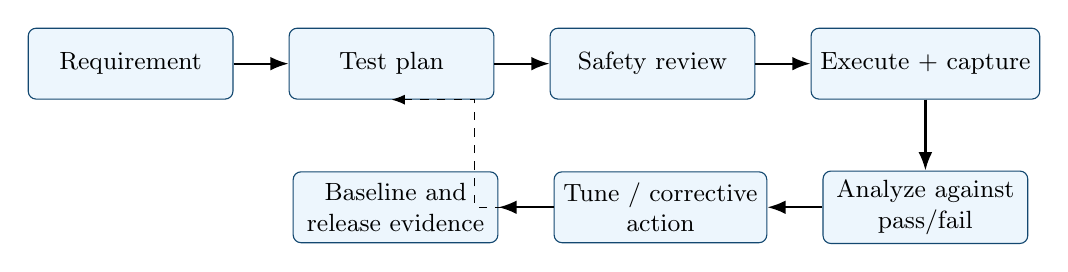
\begin{tikzpicture}[>=Latex,node distance=7mm,every node/.style={font=\small}]
\tikzset{test/.style={draw=MSBlue,fill=SoftBlue,rounded corners=1mm,minimum width=26mm,minimum height=9mm,align=center}}
\node[test] (req) {Requirement};
\node[test,right=of req] (plan) {Test plan};
\node[test,right=of plan] (safe) {Safety review};
\node[test,right=of safe] (run) {Execute + capture};
\node[test,below=9mm of run] (an) {Analyze against\\pass/fail};
\node[test,left=of an] (fix) {Tune / corrective\\action};
\node[test,left=of fix] (release) {Baseline and\\release evidence};
\draw[->,thick] (req)--(plan);
\draw[->,thick] (plan)--(safe);
\draw[->,thick] (safe)--(run);
\draw[->,thick] (run)--(an);
\draw[->,thick] (an)--(fix);
\draw[->,thick] (fix)--(release);
\draw[->,dashed] (fix.west)--++(-1,0)|-(plan.south);
\end{tikzpicture}
\caption{Closed-loop validation. Tuning without traceable evidence is not a released integration result.}
\end{figure}

\begin{longtable}{p{0.18\linewidth}p{0.25\linewidth}p{0.24\linewidth}p{0.22\linewidth}}
\toprule
Test & Stimulus & Key measurements & Pass/fail basis \\
\midrule
Steady state & Sweep $P,Q$, voltage, DC input & $V,I,P,Q$, temperature, harmonics & Accuracy, thermal, quality, and limits \\
Grid strength & Vary Thevenin $Z$, $R/X$, SCR proxy & Oscillation, PLL, current, resonance & Stable, no unwanted trips \\
LVRT & Programmed sag/profile & $V,I,V_{dc}$, states, timers & Required connection, response, recovery \\
Frequency & Step/ramp/dwell & Frequency, $P$ command/actual, limits & Droop/deadband/ramp requirements \\
Island / load step & Breaker event and load step & $V,f,I$, states, relay targets & Defined transient and restoration \\
Fault response & Controlled safe emulation & Current limit, protection sequence & Protection and coordinated response \\
Communications & Read/write/loss/reconnect & Values, timestamps, fallback mode & Mapping, permissions, safe default \\
\bottomrule
\end{longtable}

\subsection{LVRT execution example}
At the required $P/Q$ operating point, arm waveform and event capture, apply
the approved sag with a programmable grid or test source, hold for the required
time, then restore voltage. Assess voltage-measurement accuracy, current command
and actual current, priority clipping, DC-bus excursion, protection timers,
state-machine transitions, active-power recovery, and post-event oscillation.
Repeat required corners, including weak-grid conditions where applicable.

\subsection{Test data quality}
Use calibrated instruments, documented probe scaling/polarity, sufficiently high
sample rate and anti-aliasing, and synchronized timebases. Preserve raw data as
well as processed plots. The test report should tell a future engineer exactly
which configuration and instruments created each trace.

\section{Industrial Communications and Data Integrity}

\subsection{Modbus TCP and Modbus RTU}
Modbus is a request/response application protocol. Modbus TCP uses Ethernet
with TCP transport; Modbus RTU commonly uses a serial link such as RS-485.
Integration errors often arise from zero- versus one-based register notation,
16-bit register order, signed or unsigned representation, 32-bit word order,
scaling, stale data, polling load, unit ID, serial termination, and loss-of-
communications behavior. A point map must state each of these explicitly.

\subsection{CAN and SunSpec}
CAN is a multi-master message bus with identifier-based arbitration and strong
error handling. Message IDs, bit timing, termination, bus loading, and restart
behavior matter. SunSpec provides standardized information models commonly
carried over Modbus for DER equipment. Confirm the actual model/version and
vendor extensions; a claim of compatibility does not eliminate point-map or
control-authority testing.

\begin{table}[h]
\centering
\caption{Communications integration checklist}
\begin{tabular}{p{0.27\linewidth}p{0.58\linewidth}}
\toprule
Item & Verify \\
\midrule
Data semantics & Units, scale factor, sign convention, valid range, precision, endianness \\
Command authority & Local/remote state, permissions, arbitration, acknowledgment \\
Timing & Poll rate, latency, timeout, timestamp source, stale-data detection \\
Fault handling & Network loss, malformed message, reconnect, reboot, safe fallback \\
Cybersecurity & Segmentation, access control, logging, approved firmware process \\
\bottomrule
\end{tabular}
\end{table}

\subsection{Control authority and bad data}
For every command, define who has authority: local HMI, plant controller, grid
operator, commissioning tool, or inverter default. Define priority, command
acknowledgment, update rate, timeout, restart behavior, and safe fallback. Test
loss of network and malformed/stale values deliberately in a controlled setup.
A system that works only when all communications are healthy is not field-ready.

\section{Troubleshooting and Root-Cause Analysis}

\subsection{Hypothesis-driven workflow}
Do not change several parameters in response to an alarm. Preserve evidence,
define the symptom precisely, form competing hypotheses, and select the least
invasive discriminating measurement. Change one causal variable at a time where
safe. An alarm label is not root cause; a root cause explains why the event
occurred and why the corrective action prevents recurrence.

\begin{enumerate}
\item \textbf{Contain}: make the system safe; preserve logs, settings, and hardware evidence.
\item \textbf{Characterize}: state what, where, when, how often, and under what operating condition.
\item \textbf{Timeline}: align scope capture, inverter state, relay events, commands, and grid data.
\item \textbf{Hypothesize}: separate initiating event, propagation mechanism, and protection action.
\item \textbf{Discriminate}: run a test or obtain data that could prove a hypothesis wrong.
\item \textbf{Correct}: implement the narrowest robust fix and evaluate side effects.
\item \textbf{Regress}: reproduce the trigger or a bounded electrical equivalent.
\item \textbf{Prevent}: update tests, monitoring, documents, and fleet screening.
\end{enumerate}

\begin{table}[h]
\centering
\caption{Symptom-to-evidence map}
\begin{tabular}{p{0.25\linewidth}p{0.32\linewidth}p{0.31\linewidth}}
\toprule
Symptom & Candidate mechanisms & Discriminating evidence \\
\midrule
Trip during voltage sag & Timer, PLL loss, DC overvoltage, current limit & Fast $V/I/V_{dc}$, states, protection timestamps \\
Weak-grid ringing & PLL/filter/grid impedance interaction & Frequency versus grid $Z$, parameter sweep, model \\
Unexpected reactive power & Sign/scaling, volt-var, meter polarity & Raw phasors, independent meter, point map \\
Parallel sharing error & Droop mismatch, CT error, cable asymmetry & Per-unit P/Q, timing, impedance, polarity \\
Overtemperature & Derating, cooling, harmonics, poor joint & Thermal map, airflow, spectrum, inspection \\
\bottomrule
\end{tabular}
\end{table}

\subsection{Evidence-backed Five Whys}
``Why did it trip?'' may first yield ``DC overvoltage.'' Continue: why did the
DC bus rise; why did AC export collapse; why did ride-through prioritize
reactive current; why did source curtailment lag; why was this operating point
not in validation? Each answer should reference a trace, test, or controlled
reproduction. The final action may span firmware settings, source-control
timing, test coverage, and a fleet configuration audit.

\section{High-Voltage Laboratory and Field Safety}

\subsection{Energy awareness}
High voltage and high stored energy remain hazardous after a system is de-
energized. Sources include DC capacitors, batteries, rotating equipment, grid
backfeed, generators, UPS systems, and test equipment. Engineering practice
includes lockout/tagout, approved absence-of-voltage verification, discharge
time, grounding where required, arc-flash assessment, approach boundaries, and
trained personnel under site procedures.

\subsection{Safe test planning}
Before a high-energy test, define the one-line topology, energy sources,
isolation points, grounding, PPE, barriers, communication roles, emergency-stop
behavior, abort thresholds, data capture, and post-test discharge/verify steps.
Conduct a pre-job brief. Never improvise a fault or ride-through test without an
engineered method and stated equipment limits.

\begin{warningbox}{Instrumentation failure modes}
Probe insulation, current-clamp saturation, CT polarity, sensor offset, ADC
clipping, aliasing, ground loops, missing anti-alias filtering, and
unsynchronized clocks can all create convincing but false narratives.
Cross-check critical conclusions with independent measurements and known
physical limits.
\end{warningbox}

\section{Cross-Functional Engineering Interfaces}

\subsection{Mechanical and thermal}
Electrical performance depends on enclosure ingress protection, airflow,
coolant routing, cabinet layout, vibration, cable bend radius, service access,
and connector/bus-joint reliability. An electrical change can create a thermal
change: more reactive current, harmonic current, or switching frequency can
increase losses even when real power is unchanged.

\subsection{Controls and software}
Clarify ownership of state machines, command arbitration, limits, faults,
parameter units, default values, version compatibility, and rollback. For a
firmware change, require release notes, configuration migration behavior, test
evidence, telemetry compatibility, and a recovery plan. System behavior lives
at the boundary between controls and hardware; neither discipline validates that
boundary alone.

\subsection{Manufacturing and quality}
Design reviews should consider tolerance stack-up, CT/PT polarity and wiring,
torque-controlled joints, insulation clearances, harness routing, test points,
end-of-line validation, traceability, and service diagnostics. A robust
integration design is testable and observable at production scale, not merely
functional on one development unit.

\section{Worked System-Integration Study}

Consider a $1.0\,\MW$ generation asset connected through an OTS inverter to a
$480\,V$ AC collection bus. It must export at PF $=0.90$, provide voltage
support, remain connected through a defined sag, and operate over a range of
source impedance.

At the specified power factor, required apparent and reactive power are
\[
S=1.111\,\MVA,\qquad Q=0.484\,\Mvar,
\]
and line current is $1337\,\A$. This establishes the current scale but must be
combined with environmental derating, continuous and overload requirements,
harmonic current, fault duty, and terminal ratings.

If available three-phase POI fault level is $10\,\MVA$, then the preliminary
grid-strength screen is
\[
SCR\approx\frac{10}{1.111}=9.0.
\]
This is not a stability guarantee. Gather source impedance and $R/X$ range,
transformer/feeder data, parallel equipment, and the inverter's documented
stability envelope. Validate worst credible conditions using a programmable
grid or representative network.

The configuration baseline needs GFL/GFM availability, PLL and droop settings,
P/Q priorities, current limits, ride-through curves, protection settings,
communications authority, and firmware revision. Test steady-state operation,
grid-strength variation, LVRT, frequency response, communications loss,
protection response, and recovery. Each report plot must include configuration
and instrument context so it can be reproduced.

Suppose a 12 Hz P/Q oscillation appears only at a remote site and low real
power. Do not tune random gains. Compare site source impedance and voltage-
control devices; align P/Q, PLL, voltage, current, and command data; then
reproduce with increased grid impedance. Candidate mechanisms include PLL
interaction, outer-loop interaction, volt-var/regulator hunting, and a
communications setpoint loop. Change one candidate path while holding the
operating point and measurement method fixed; this is a discriminating test.

\section{Formula Sheet and Release Checklist}

\begin{longtable}{p{0.35\linewidth}p{0.54\linewidth}}
\toprule
Topic & Key relation / reminder \\
\midrule
Instantaneous power & $p(t)=v(t)i(t)$ \\
RMS & $X_{rms}=\sqrt{\frac1T\int_0^T x^2(t)dt}$ \\
Energy storage & $E_C=\frac12CV^2$; $E_L=\frac12LI^2$ \\
Complex power & $\underline S=\underline V\underline I^*=P+\jop Q$ \\
Three-phase power & $P=\sqrt3V_{LL}I_L\cos\phi$; $Q=\sqrt3V_{LL}I_L\sin\phi$ \\
Apparent-power limit & $P^2+Q^2\le S_{max}^2$ \\
Base quantities & $I_B=S_B/(\sqrt3V_{B,LL})$; $Z_B=V_{B,LL}^2/S_B$ \\
Grid model & $\underline V_{POI}=\underline V_{th}-\underline I\underline Z_{th}$ \\
Grid strength & $SCR=S_{sc}/S_{inv}$ \\
Three-phase fault & $I_{3\phi}=V_{LL}/(\sqrt3|Z_{th}|)$ \\
LCL resonance & $f_r=(2\pi)^{-1}\sqrt{(L_1+L_2)/(L_1L_2C_f)}$ \\
GFM droop & $\omega=\omega_0-m_p(P-P_0)$; $V=V_0-n_q(Q-Q_0)$ \\
Current limit & $i_d^{*2}+i_q^{*2}\le i_{max}^2$ \\
Harmonics & $THD=\sqrt{\sum_{h\ge2}X_h^2}/X_1\times100\%$ \\
Thermal estimate & $T_j=T_a+P_{loss}\sum R_\theta$ \\
\bottomrule
\end{longtable}

\begin{checklistbox}{Before release or field deployment}
\begin{itemize}
\item Verify ratings, derating, transformer connection, grounding, and fault duty for the installed topology.
\item Control inverter mode, firmware, parameters, protection, and communications-map revisions.
\item Validate GFL/GFM behavior across required P/Q, DC voltage, grid voltage/frequency, and impedance conditions.
\item Capture traceable evidence for ride-through, frequency response, voltage/reactive functions, protection, and recovery.
\item Evaluate thermal behavior, power quality, transients, safety procedures, and field diagnostics.
\item Give every open risk an owner, due date, mitigation, and regression or monitoring plan.
\end{itemize}
\end{checklistbox}

\begin{keybox}{Systems-engineering mindset}
Connect a model to a measurement and a decision: ``The weak feeder increases
source impedance and reduces stability margin; vary programmed grid impedance,
capture PLL/current behavior, tune within the vendor-approved envelope, and
verify ride-through and recovery with the released configuration.'' That is how
electrical fundamentals become reliable inverter-system integration.
\end{keybox}

\end{document}